\begin{frame}{4. Evaluation: Benchmark}

  \begin{itemize}
  \item \textbf{Numerical Differentiation} for experimental data
    \begin{itemize}
    \item 1D stencil computation, sensitive to computation accuracy
    \end{itemize}
  \item \textbf{Black Scholes} for finite difference option pricing
    \begin{itemize}
    \item 1D stencil, multiple time steps, requires DRAM
    \end{itemize}
  \item \textbf{Reverse Time Migration} for seismic imaging
    \begin{itemize}
    \item 3D stencil, design parallelism, operator tuning
    \end{itemize}
  \item \textbf{Bitonic Network} for high-throughput sorting
    \begin{itemize}
    \item recursive definition, design parametrisation
    \end{itemize}
  \item \textbf{Add Prediction} for Bing's sponsored search
    \begin{itemize}
    \item arithmetic intensive kernel
    \item requires effective tuning to achieve timing closure
    \end{itemize}
  \end{itemize}
\end{frame}

\begin{frame}{4. Evaluation: Reverse Time Migration}
  \begin{itemize}
  \item seismic imaging application for oil and gas exploration
  \item 3 dataflow kernels
    \begin{itemize}
    \item RTM -- compute intensive, multiple configurations
    \item CmdWrite -- memory write command generator
    \item CmdRead -- memory read command generator
    \end{itemize}
  \item computationally demanding
  \item use run-time reconfiguration to improve performance and efficiency
  \end{itemize}
\end{frame}


\begin{frame}{4. Evaluation: RTM Design Space Exploration}
  \begin{figure}[!h]
    \centering
    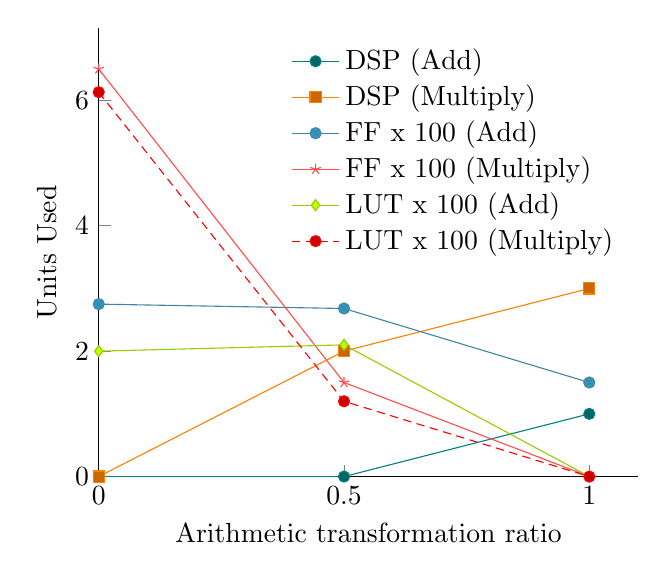
\begin{tikzpicture}
      \begin{axis}[
        cycle list name=exotic,
        xmin=0,
        ymin=0,
        axis y line*=left,
        axis x line* =bottom,
        xlabel=Arithmetic transformation ratio,
        ylabel=Units Used,
        xtick={0, 0.5, 1},
        legend columns=1,
        legend entries={
          DSP (Add),
          DSP (Multiply),
          FF x 100 (Add),
          FF x 100 (Multiply),
          LUT x 100 (Add),
          LUT x 100 (Multiply),
        },
        legend style={
          draw=none,
          cells={anchor=west}
        }
        ]
        \addplot coordinates {
          (0, 0)
          (0.5, 0)
          (1, 1)
        };
        \addplot coordinates {
          (0, 0)
          (0.5, 2)
          (1, 3)
        };
        \addplot coordinates {
          (0, 2.75)
          (0.5, 2.68)
          (1, 1.50)
        };
        \addplot coordinates {
          (0, 6.5)
          (0.5, 1.5)
          (1, 0)
        };
        \addplot coordinates {
          (0, 2)
          (0.5, 2.1)
          (1, 0)
        };
        \addplot coordinates {
          (0, 6.13)
          (0.5, 1.2)
          (1, 0)
        };
      \end{axis}
    \end{tikzpicture}
  \end{figure}
\end{frame}

\begin{frame}{4. Evaluation: RTM Word Length Exploration}
  \begin{figure}
    \centering
    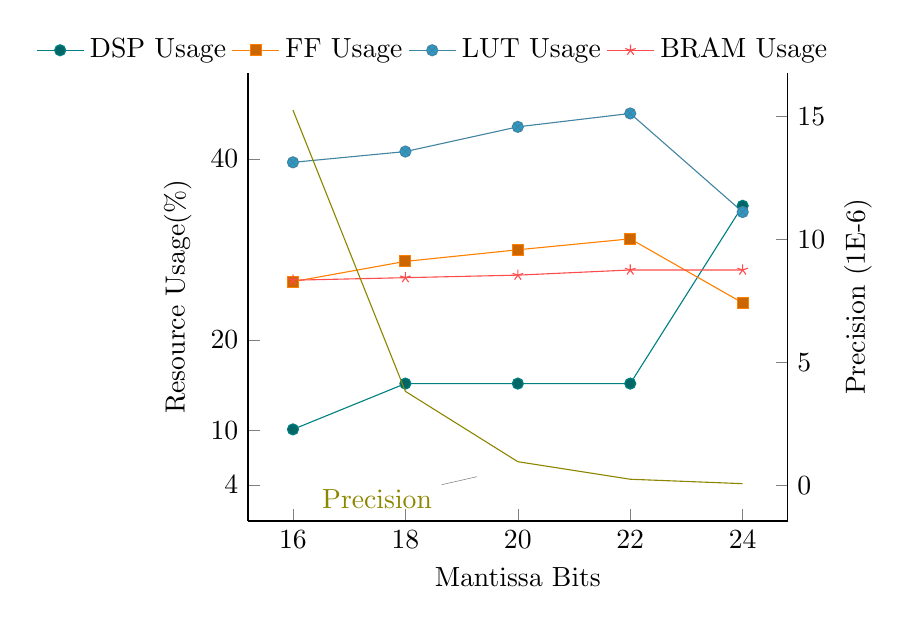
\begin{tikzpicture}
      \begin{axis}[
        cycle list name=exotic,
        ymin=0,
        axis y line*=left,
        axis x line*=bottom,
        xlabel=Mantissa Bits,
        ylabel=Resource Usage(\%),
        xtick=data,
        ytick={4, 10, 20, 40, 50, 70, 80, 100},
        legend columns=4,
        legend entries={
          DSP Usage,
          FF Usage,
          LUT Usage,
          BRAM Usage},
        legend style={
          draw=none,
          anchor=east,
          at={(1.1, 1.05)}
        }
        ]
        \addplot coordinates {
          (24, 34.82)
          (22, 15.18)
          (20, 15.18)
          (18, 15.18)
          (16, 10.12)
        };
        \addplot coordinates {
          (24, 24.09)
          (22, 31.17)
          (20, 29.96)
          (18, 28.68)
          (16, 26.44)
        };
        \addplot coordinates {
          (24, 34.13)
          (22, 45.02)
          (20, 43.54)
          (18, 40.81)
          (16, 39.62)
        };
        \addplot coordinates {
          (24, 27.73)
          (22, 27.73)
          (20, 27.16)
          (18, 26.88)
          (16, 26.60)
        };
      \end{axis}
      \begin{axis}[
        ylabel=Precision (1E-6),
        axis y line*=right,
        axis x line=none,
        ]
        \addplot[color=olive] coordinates {
          (16, 15.2585)
          (18, 3.8146)
          (20, 0.9536)
          (22, 0.2394)
          (24, 0.0596)
        } node [pos=0.8,pin={190:Precision},inner sep=20pt] {};
      \end{axis}
    \end{tikzpicture}
  \end{figure}
\end{frame}

\begin{frame}{4. Evaluation: RTM Parallelism}
  \begin{figure}[!h]
    \centering
    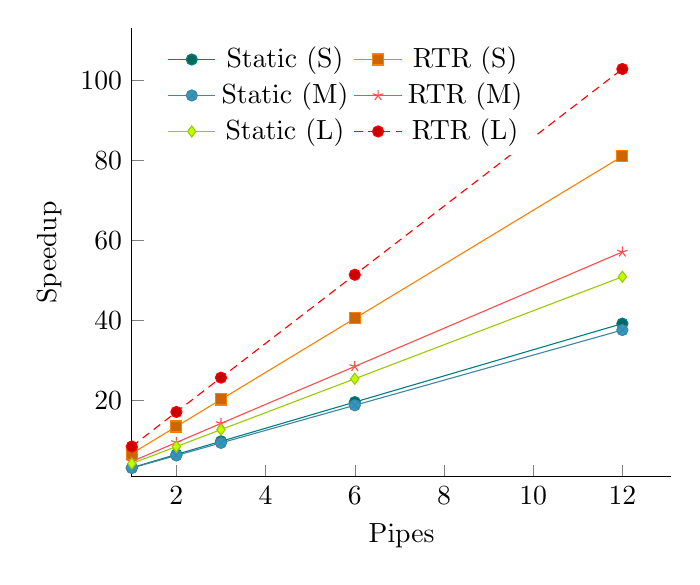
\begin{tikzpicture}
      \begin{axis}[
        cycle list name=exotic,
        xmin=1,
        ymin=1,
        xlabel=Pipes,
        ylabel=Speedup,
        axis x line* =bottom,
        axis y line* = left,
        legend columns=2,
        legend entries={
          Static (S),
          RTR (S),
          Static (M),
          RTR (M),
          Static (L),
          RTR (L)},
        legend style={
          draw=none,
          at={(0.05,0.85) },
          anchor=west
        }
        ]
        \addplot coordinates {
          (1, 3.2)
          (2, 6.53)
          (3, 9.8)
          (6, 19.6)
          (12, 39.2)
        };
        \addplot coordinates {
          (1, 6.75)
          (2, 13.5)
          (3, 20.25)
          (6, 40.5)
          (12, 81)
        };
        \addplot coordinates {
          (1, 3.13)
          (2, 6.26)
          (3, 9.4)
          (6, 18.8)
          (12, 37.6)
        };
        \addplot coordinates {
          (1, 4.75)
          (2, 9.51)
          (3, 14.27)
          (6, 28.5)
          (12, 57.1)
        };
        \addplot coordinates {
          (1, 4.25)
          (2, 8.48)
          (3, 12.725)
          (6, 25.42)
          (12, 50.9)
        };
        \addplot coordinates {
          (1, 8.5)
          (2, 17.13)
          (3, 25.7)
          (6, 51.4)
          (12, 102.8)
        };
      \end{axis}
    \end{tikzpicture}
  \end{figure}
\end{frame}


\begin{frame}{4. Evaluation: Reverse Time Migration}
  Evaluation results show that aspect descriptions can effectively:
  \begin{itemize}
  \item control DSP mapping: explore trade-off of reducing LUT/FF usage,
    improving timing, reducing build time vs increasing parallelism (when DSP bound)
  \item control word length: explore improving computation accuracy vs
    reducing resource usage (also increasing parallelism)
  \item explore design space to reveal unintuitive results that can
    lead to substantial (2X) performance increase with minimal impact
    on accuracy (when reducing mantissa from 24 bits to 22 bits)
  \item control design parallelism: explore increased performance vs
    increased compilation time
  \end{itemize}
\end{frame}

\begin{frame}{4. Evaluation: Reverse Time Migration}
  \begin{table}

  \end{table}
\end{frame}

\begin{frame}{4. Evaluation: Benchmark}
  Comparing manual MaxCompiler designs to FAST designs:
  \begin{table}
    \renewcommand{\arraystretch}{1.2}
    \begin{tabular}{l|p{1cm}|p{1cm}|c|p{2cm}}
      \textbf{Kernel} & \textbf{LOC} & \textbf{API Calls} & \textbf{Performance}              & \textbf{Resource}
      \\
      \hline\hline
      CmdRead         & 1.76               & 4.33                     & \multirow{2}{*}{$ > 75\%$}        & \multirow{6}{3cm}{$\approx 100\%$} \\
      CmdWrite        & 1.45               & 4.13                     &                                   &                              \\
      \cline{1-4}
      RTM             & 1.17               & 10                       & \multirow{5}{*}{$ \approx 100\%$} &                              \\
      SGSmooth        & 1.85               & 14                       &                                   &                              \\
      SGDifff         & 1.75               & 14                       &                                   &                              \\
      Black-Scholes   & 2.51               & 5.5                      &                                   &                              \\
      \cline{5-5}
      Add Prediction  & 1.67               & 16                       &                                   &    $ \approx 123 \% $                          \\
    \end{tabular}
  \end{table}

\end{frame}